\subsubsection{Output Signal of Inverter Circuit}

The inverter circuit is constructed using a BJT. The input and output signals of the BJT inverter circuit are analyzed to determine its unique properties. The output signal is taken from the collector of the BJT in the circuit, which can be visualized below:

\FloatBarrier
\begin{figure}[h!]
	\centering
	\caption{BJT Inverter Circuit}
	\label{fig:bjt_inverter}
	\begin{circuitikz}
		\draw
		( 0 , 0 ) node[ npn ] (my_npn) {$V_{out}$}
		
		% Base
		(my_npn.B) to [ short ] +( -2 , 0 ) coordinate(r_in)
		(r_in) to [ R={$10k\Omega$} ] ++( -2 , 0 ) coordinate(v_in)
		(v_in) to [ sqV , v<=$V_{in}$ ] ++( 0 , -2 ) coordinate(gnd_1)
		(gnd_1) node[ ground ] (my_gnd_1) {}
		
		% Collector
		(my_npn.C) to [ short ] ++( 0 , 2 ) coordinate(r_c)
		(r_c) to [ R={$1k\Omega$} ] ++( 0 , 2 ) coordinate(vcc)
		(vcc) to [ battery , v<=$V_{cc}$ ] ++( 2 , 0 ) coordinate(gnd_3)
		(gnd_3) node[ ground ] (my_gnd_3) {}
		
		% Emitter
		(my_npn.E) to [ short ] ++( 0 , -2 ) coordinate(e_gnd)
		(e_gnd) node[ ground ] (my_e_gnd) {}
		
		;
	\end{circuitikz}
\end{figure}

\FloatBarrier

By supplying the inverter with a $10$\si{\kilo\hertz} square input signal with fixed minimum and maximum values at $0$\si{\volt} and $5$\si{\volt} respectively with a $50\%$ duty cycle and a $V_{cc}$ value of $5$\si{\volt}, the following input and output signals are observed on the oscilloscope:

\FloatBarrier
\begin{figure}[h!]
	\centering
	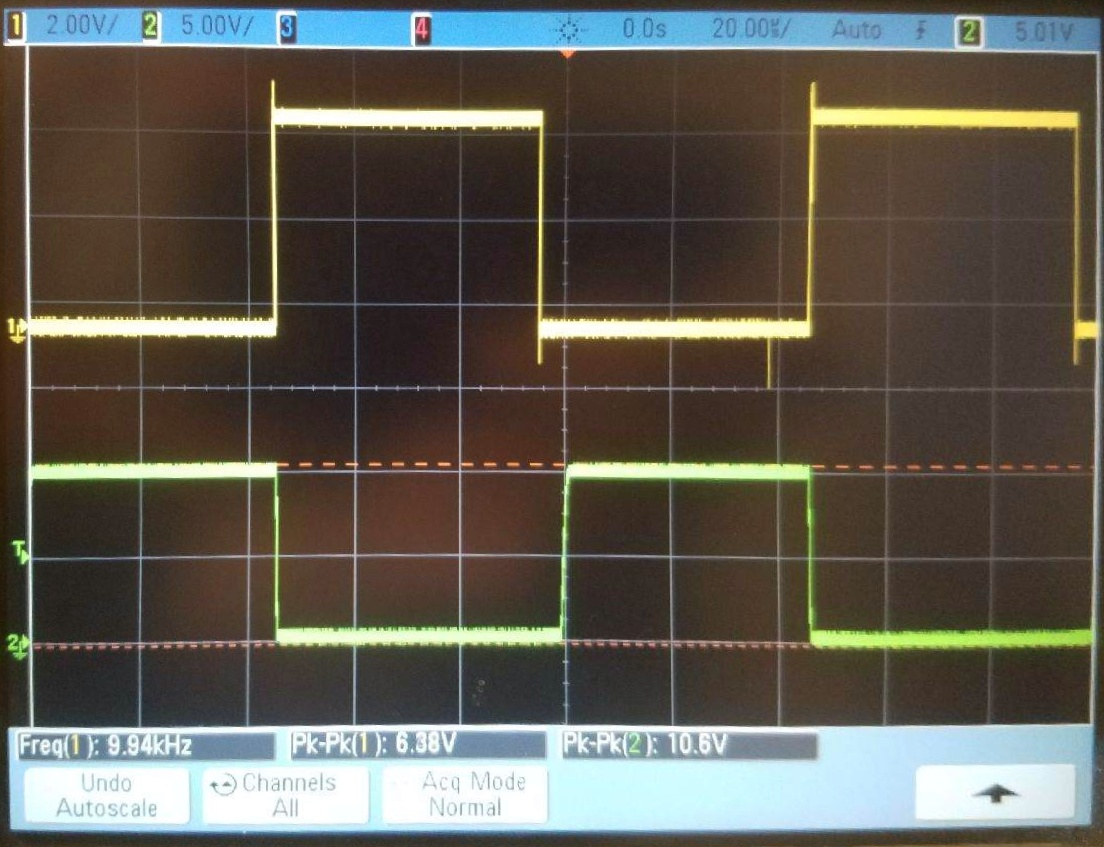
\includegraphics[scale=0.25]{../images/inverter_input_output.jpeg}
	\caption{Input and Output Signals of BJT Inverter}
	\label{fig:inverter_in_out}
\end{figure}
\FloatBarrier

When the square source is at its maximum, a large voltage is supplied to the base of the BJT. This translates to a forward-bias applied across the base-emitter junction and base-collector junction. At this point the BJT is operating in the saturation region. In the saturation region, the transistor effectively acts as a short circuit thus causing the output voltage at the emitter to be zero.

When the square source is at its minimum, essentially no voltage is supplied to the base of the BJT. As a result, the base-emitter junction and the base-collector junction are reverse biased and the BJT is operating in the cutoff region. In the cutoff region, the transistor effectively acts as an open circuit, so the output voltage at the emitter is equivalent to the value of $V_{cc}$.

By zooming in to the output signal, the rise and fall time of the signal can be measured.

\FloatBarrier
\begin{figure}[h!]
	\centering
	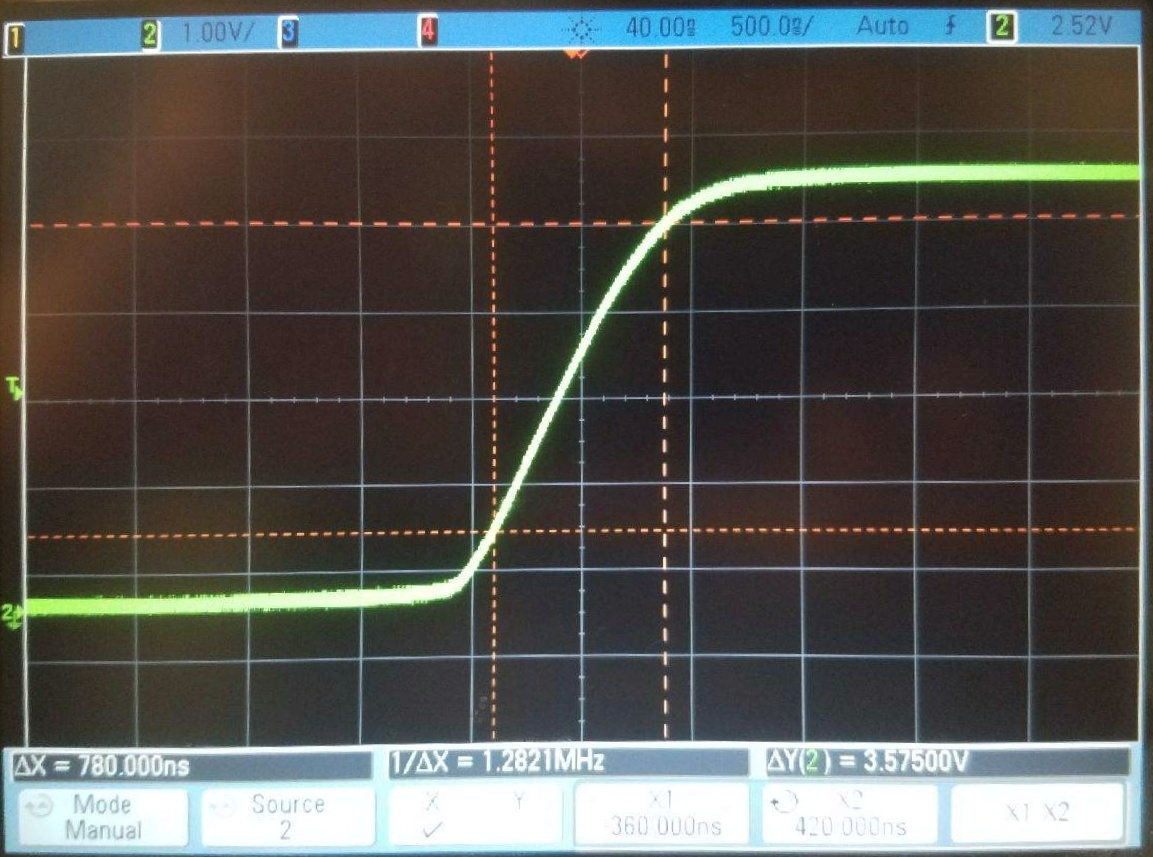
\includegraphics[scale=0.24]{../images/inverter_tr.jpeg}
	\caption{Rise Time of Output Signal}
	\label{fig:inverter_tr}
\end{figure}
\FloatBarrier

The rise time is found by measuring the difference in time of when the signal reaches $10\%$ of its relative maximum and when the signal reaches $90\%$ of its relative maximum at the rising edge. Using this method, the rise time of the output signal, $t_r$ is measured to be $780$\si{\nano\second}.

\FloatBarrier
\begin{figure}[h!]
	\centering
	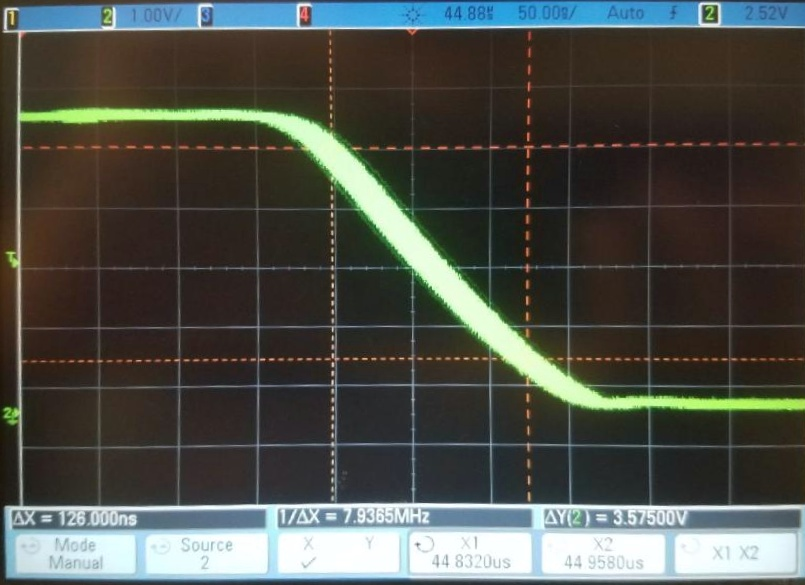
\includegraphics[scale=0.34]{../images/inverter_tf.jpeg}
	\caption{Fall Time of Output Signal}
	\label{fig:inverter_tf}
\end{figure}
\FloatBarrier

The fall time is found by measuring the difference between the time in which the signal reaches $90\%$ of its relative maximum and the time in which the signal reaches $10\%$ of its relative maximum at the falling edge. Using this method, the fall time of the output signal, $t_f$ is measured to be $126$\si{\nano\second}.

The delay times between the input and output signals for the saturation to cutoff transition and the cutoff to saturation transition of the BJT can be found by finding the difference between the time in which the input and output signals reach $50\%$ of their respective relative maxima. The measurement taken for the delay time for the saturation to cutoff transition of the BJT is shown in the following figure:

\FloatBarrier
\begin{figure}[h!]
	\centering
	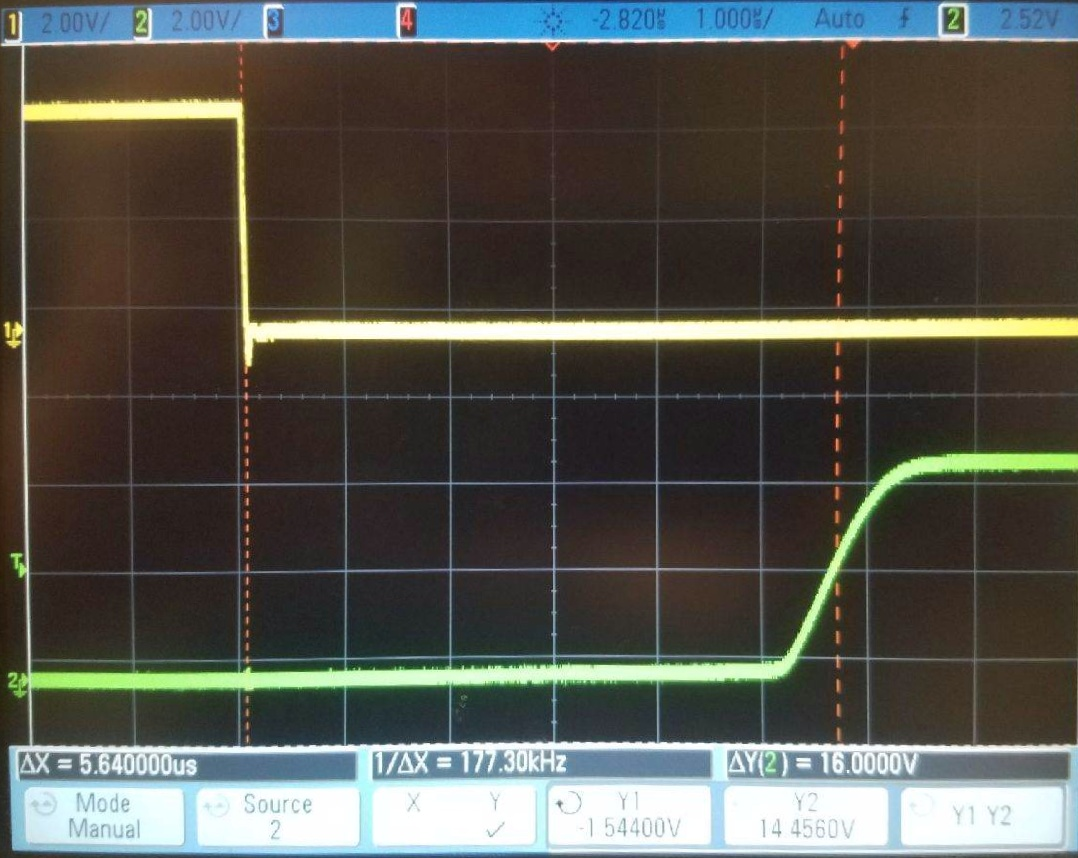
\includegraphics[scale=0.26]{../images/inverter_td.jpeg}
	\caption{Delay Time for Saturation to Cutoff Transition}
	\label{fig:inverter_td}
\end{figure}
\FloatBarrier

The delay time, $t_d$, for the saturation to cutoff transition of the BJT is measured to be $5.64$\si{\micro\second}. $t_d$ for the cutoff to saturation transition of the BJT is very close to the value found for $t_f$, and is approximately $130$\si{\nano\second}. The $t_d$ value for the saturation to cutoff transition is the more significant one by a large margin.

While the delay times are large for the BJT inverter circuit, they are still reasonable at $10$\si{\kilo\hertz}. This is because at $10$\si{\kilo\hertz}, the period of the wave is $0.1$\si{\milli\second}. The maxima and minima of a square wave at that frequency would then have a duration of $50$\si{\micro\second} which is significantly larger than the delay times, meaning their effects are relatively minimal. However, for high frequency applications, the BJT inverter circuit will fail. If the input signal has a frequency of $3$\si{\giga\hertz}, then the period of the wave would be $0.333$\si{\nano\second}. The delay times of the BJT inverter are orders of magnitudes larger than the period of the wave. Inversion of the input signal would not be observed because the slow switching time of the BJT.